\documentclass[a4paper]{article}
\usepackage[final]{pdfpages}

\addtolength{\textheight}{3cm}
\addtolength{\voffset}{-.8cm}

\begin{document}
\pagenumbering{arabic}
\setcounter{page}{1}

\title{Curso 2: Generaci\'on de Lenguaje Natural y Aplicaciones}
\author{Carlos Areces\\
  {\tt carlos.areces@gmail.com} 
\and 
Luciana Benotti\\
  {\tt Luciana.Benotti@gmail.com} \\
 \ \\
  Equipo TALARIS - INRIA Nancy Grand Est - Francia\\
  Equipo PLN - Universidad Nacional de C\'ordoba - Argentina
}


\maketitle

Este curso est\'a compuesto por dos partes. En la primera se dar\'a una introducci\'on al problema de generaci\'on de lenguaje natural. Presentaremos los algoritmos cl\'asicos de generaci\'on, haciendo \'enfasis en la generaci\'on de referencias. En la segunda parte discutiremos sistemas de generaci\'on situados en un entorno virtual.

La segunda parte tiene como requisito previo la primera. La evaluaci\'on final cubrir\'a temas de ambas partes.

\section*{Primera Parte: Introducci\'on a la Generaci\'on de Lenguaje Natural}

\paragraph{Profesor:} Carlos Areces (INRIA Grand Est, Francia / Univ. Nacional de C\'ordoba)

\paragraph{Horario:} Lunes, martes y mi\'ercoles de 14 a 17 hs (9 horas de clase)

\paragraph{Pre-requisitos:} Conocimientos b\'asicos de l\'ogica y algoritmos. No se asume conocimiento previo de procesamiento de lenguaje natural.

El problema de generaci\'on de lenguaje natural puede definirse, intuitivamente, como el proceso de transformaci\'on de informaci\'on en texto (escrito o hablado) en lenguaje natural (por ejemplo, Ingl\'es o Español). El texto generado debe ser no solamente gramaticalmente correcto, sino adecuado para el contexto en donde ser\'a utilizado.

\subsection*{Lunes:} El Problema de Generaci\'on de Lenguaje Natural (GLN). Historia. Generaci\'on vs. Parsing. GNL Pipeline. Representaci\'on de Informaci\'on e Inferencia para GLN. Evaluaci\'on de Sistemas de GLN.

\subsection*{Martes:} Generaci\'on Sint\'actica. Generaci\'on via Charts. Tree Adjoining Grammars. Interface Sint\'actica-Sem\'antica.

\subsection*{Mi\'ercoles:} Algoritmos de Generaci\'on de Expresiones Referenciales. Informaci\'on Proposicional vs. Informaci\'on Relacional. Optimizaci\'on de Algoritmos. Evaluaci\'on.


\section*{Segunda Parte: Generaci\'on de Instrucciones en un Entorno Virtual}

\paragraph{Profesora:} Luciana Benotti (INRIA Grand Est, Francia / Univ. Nacional de C\'ordoba)

\paragraph{Horario:} Jueves y viernes de 14 a 17 hs (6 horas de clase)

\paragraph{Pre-requisitos:} Primera parte

En esta parte del curso nos enfocaremos en sistemas de generaci\'on que tienen como objetivo una tarea concreta y que est\'an situados en un entorno 3D. Analizaremos como estas dos caracter\'isticas tienen impacto en las estrategias de generaci\'on de lenguaje natural.

\subsection*{Jueves:} Entornos Virtuales (e.g., Second Life) y Aplicaciones (e.g., Tutoring) para Sistemas de GNL. Inferencia Orientada a Metas. Algoritmos de Planning y su uso en Entornos Virtuales.

\subsection*{Viernes:} Generaci\'on de Referencias en un Entorno Virtual. Estrategias de Referencia. Supervisi\'on de la Interpretaci\'on. Evaluaci\'on.


\label{planning-state-search} 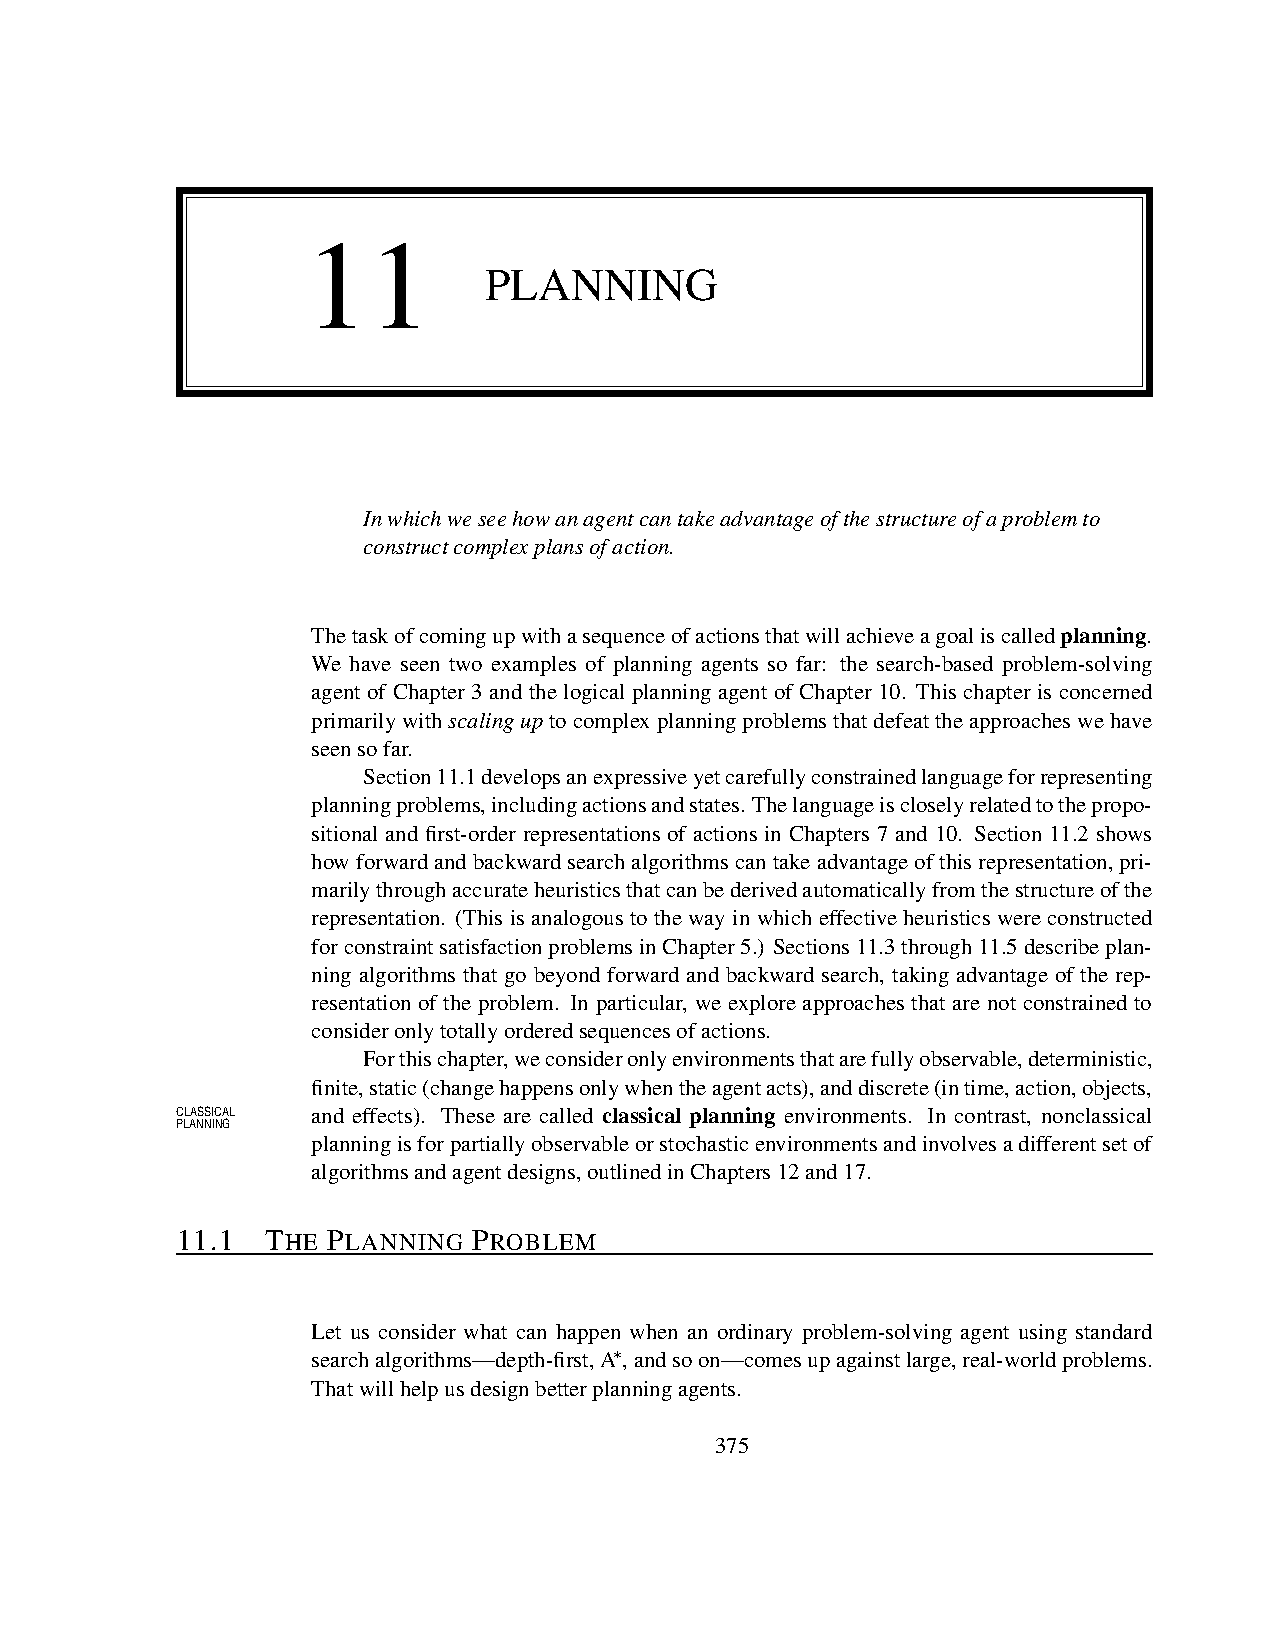
\includepdf[nup=1x2, landscape, pages={1-13}, scale=.92, frame, pagecommand={}]{russell-norvig-chap11.pdf}
\label{planning-graphplan} \includepdf[nup=1x2, landscape, pages={21-28}, scale=.92, frame, pagecommand={}]{russell-norvig-chap11.pdf}
\label{planning-history} \includepdf[nup=1x2, landscape, pages={34-38}, scale=.92, frame, pagecommand={}]{russell-norvig-chap11.pdf}
\label{give-challenge} 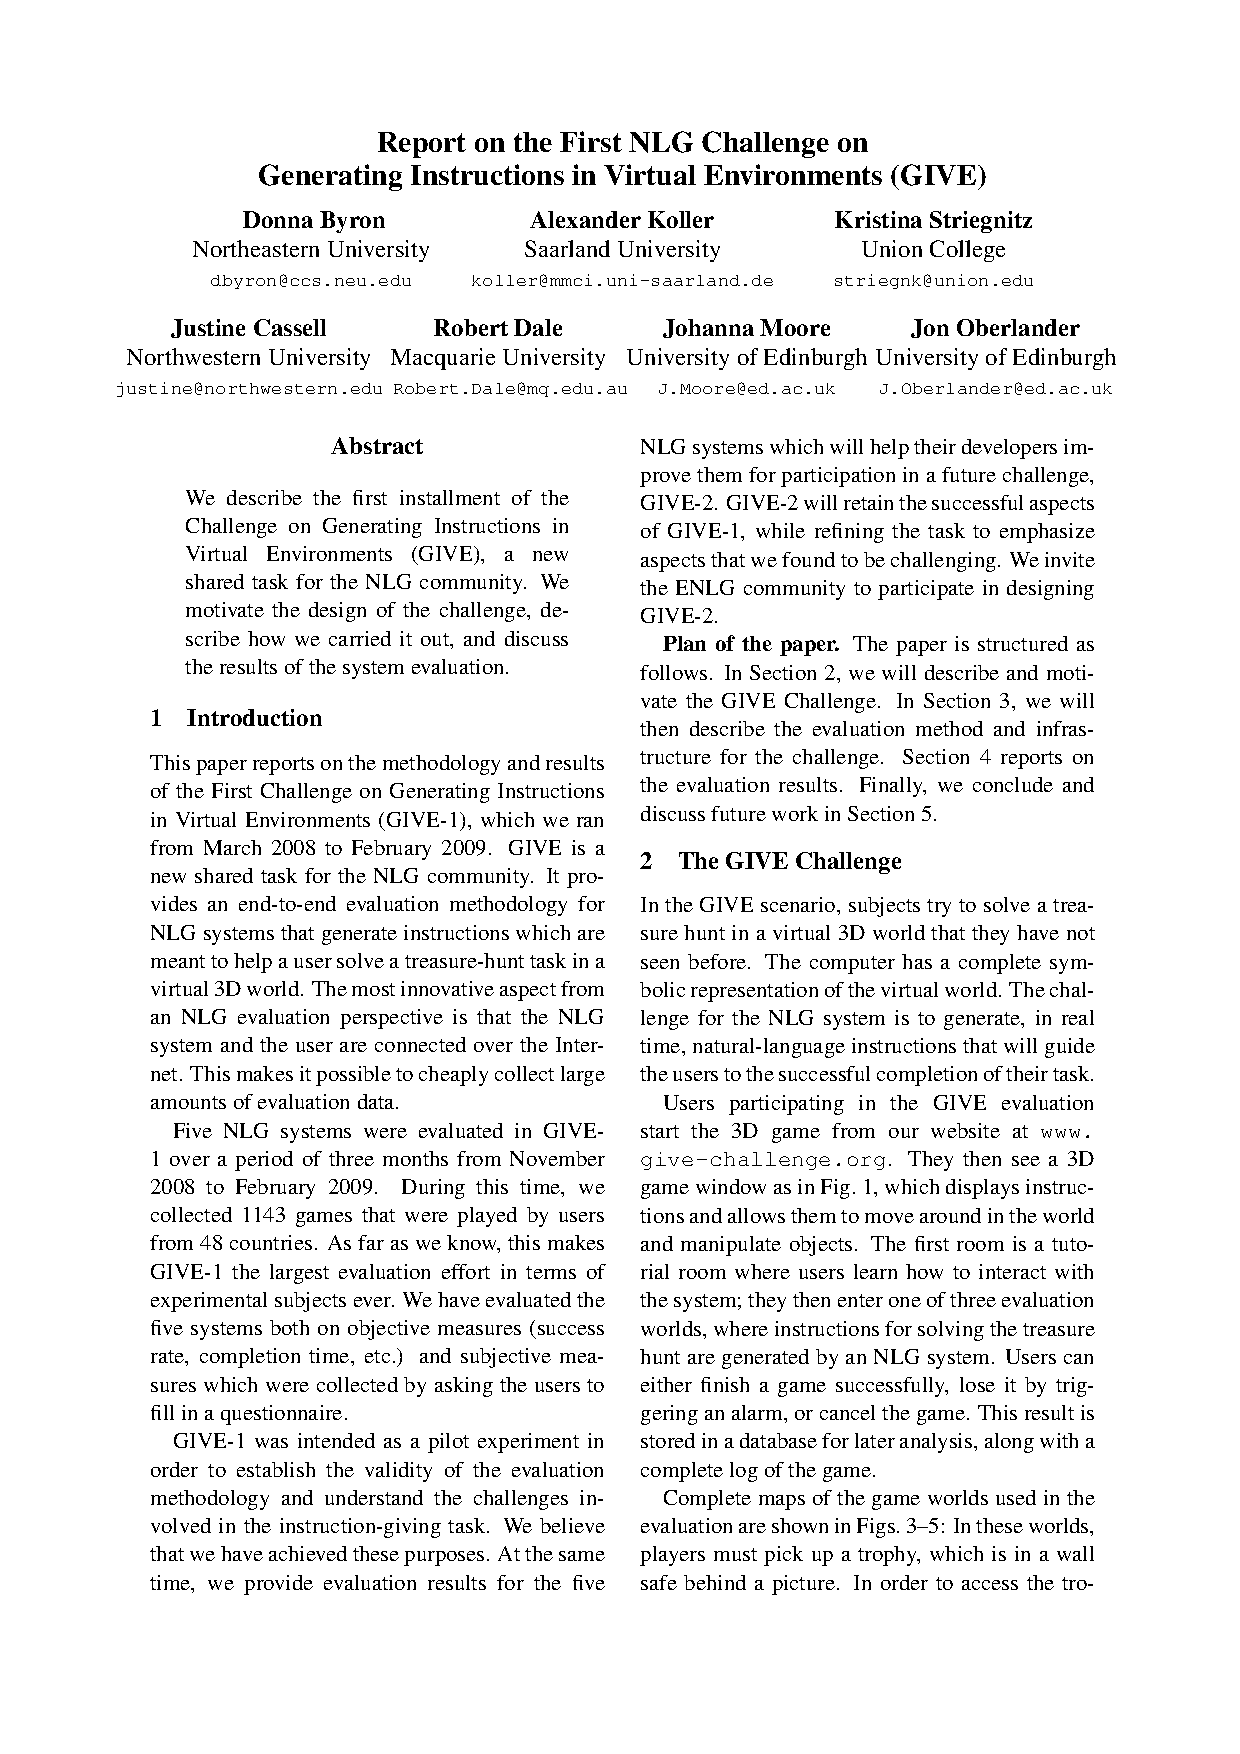
\includepdf[pages={1-9}, scale=.92, frame, pagecommand={}]{give-report-09.pdf}
\label{situated-REG} 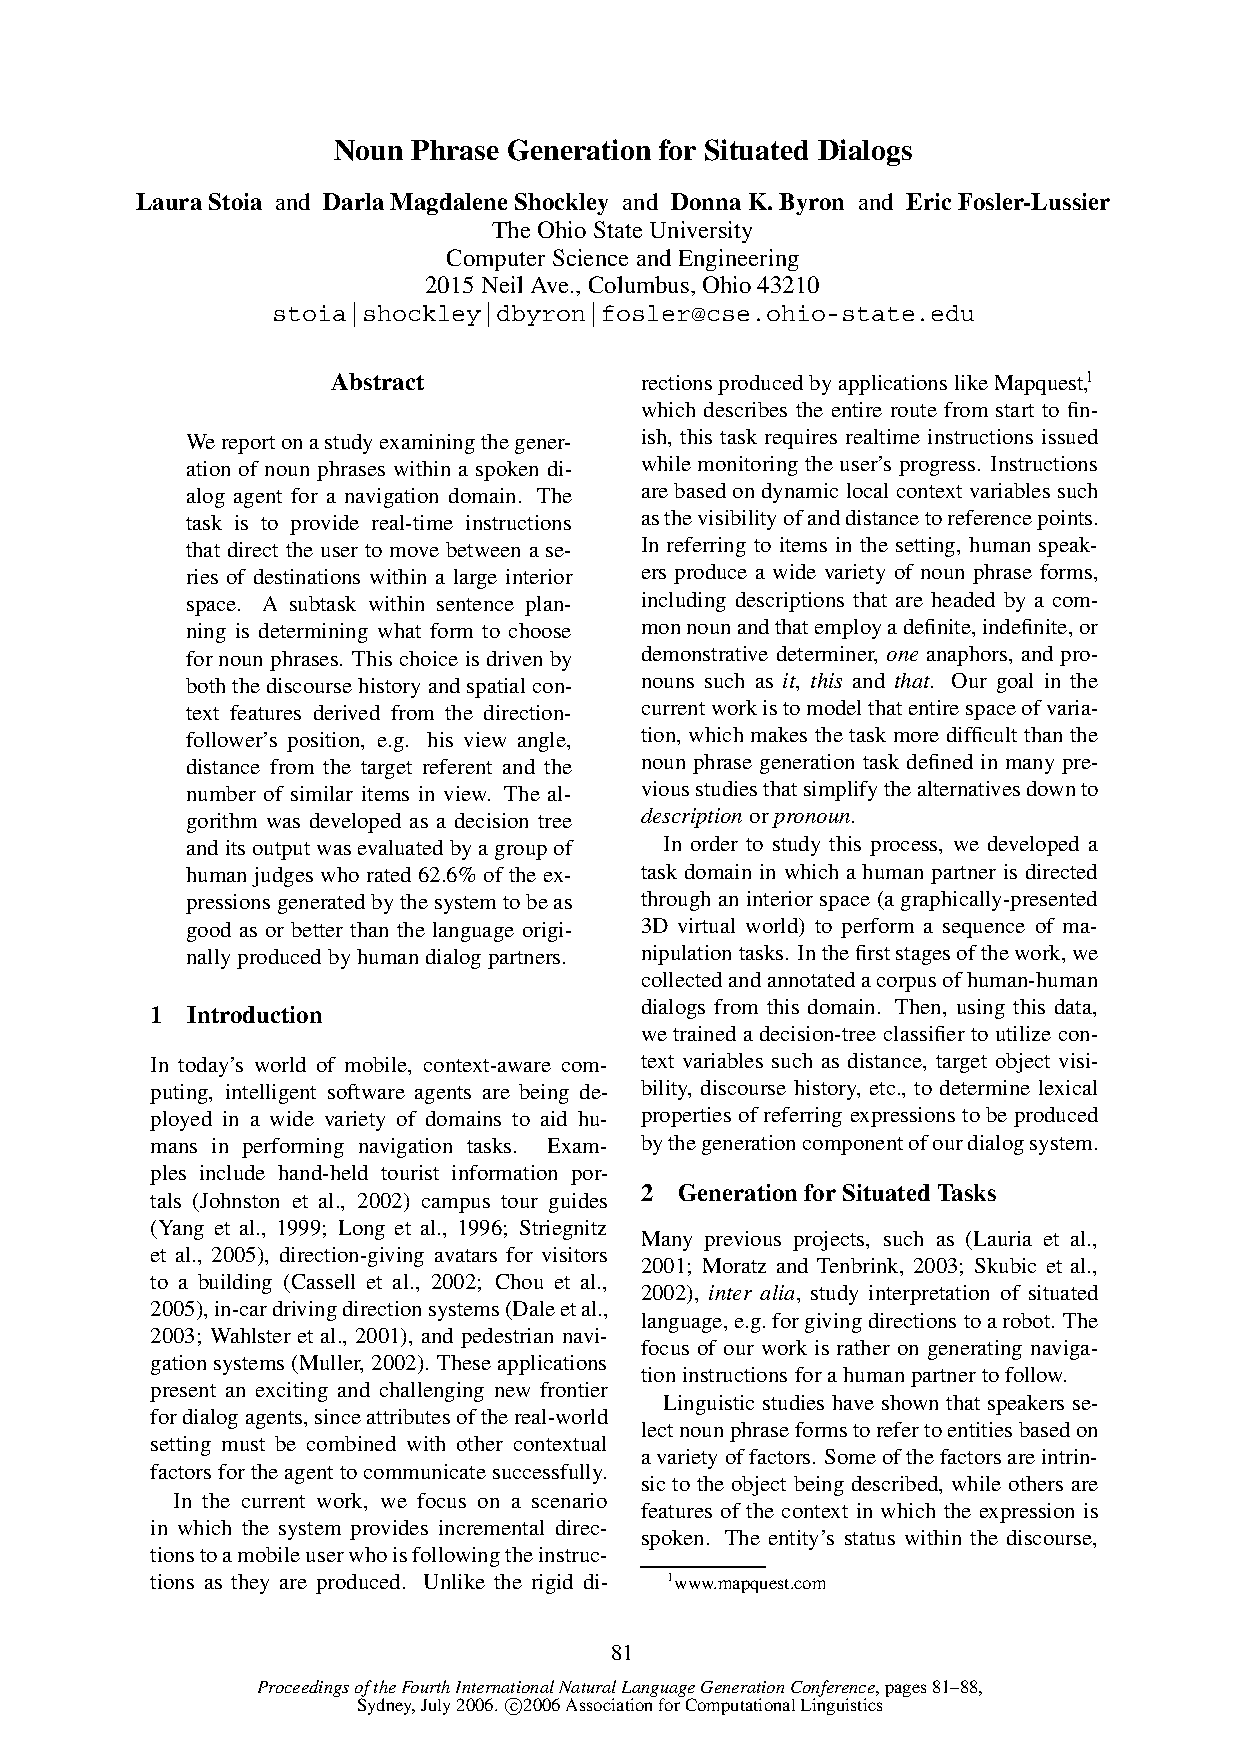
\includepdf[pages={1-8}, scale=.92, frame, pagecommand={}]{Situated-REG.pdf}

\end{document}
